\subsection{Memory}\label{subsec: ola-memory}
The memory structure of OlaVM consists of two types(Read-Write and Write-Once) and mapping to disjoint regions of the memory space.
\begin{table}[!ht]
    \resizebox{\textwidth}{!}{
        \begin{tabular}{|c|c|c|}
            \hline
            \textit{Memory Seg}  & \textit{Type} & \textit{Range}  \\ \hline
            random access memory & Read-Write &  $[0,  2^{64}-3\cdot 2^{32}-1] $ \\ \hline
            ecdsa & Write-Once &  $[2^{64}-3\cdot 2^{32}, 2^{64}-2\cdot 2^{32}-1] $ \\ \hline
            poseidon & Write-Once &  [$2^{64}-2\cdot 2^{32},  2^{64}- 2^{32}-1] $ \\ \hline
            prophet & Write-Once &  $[2^{64}-2^{32}, 2^{64}-1]$ \\ \hline
        \end{tabular}}
    \caption{Memory segment range}
    \label{table:memory-segment-range}
\end{table}


OlaVM use B-Tree algorithm to manage the memory address, support random access memory.B-Tree algorithm sort the memory by address and cpu clock when insert data to the memory bu address.
\begin{enumerate}
    \item when random access memory, the time complexity of search is $\texttt{O(logN)}$.
    \item when generate memory trace table by address and clock in ascending order,the memory can direct visit, not need sort again.
\end{enumerate}

The memory structure illustration is as below \ref{fig: B-tree-memory}:
\begin{figure}[!htp]
    \centering
    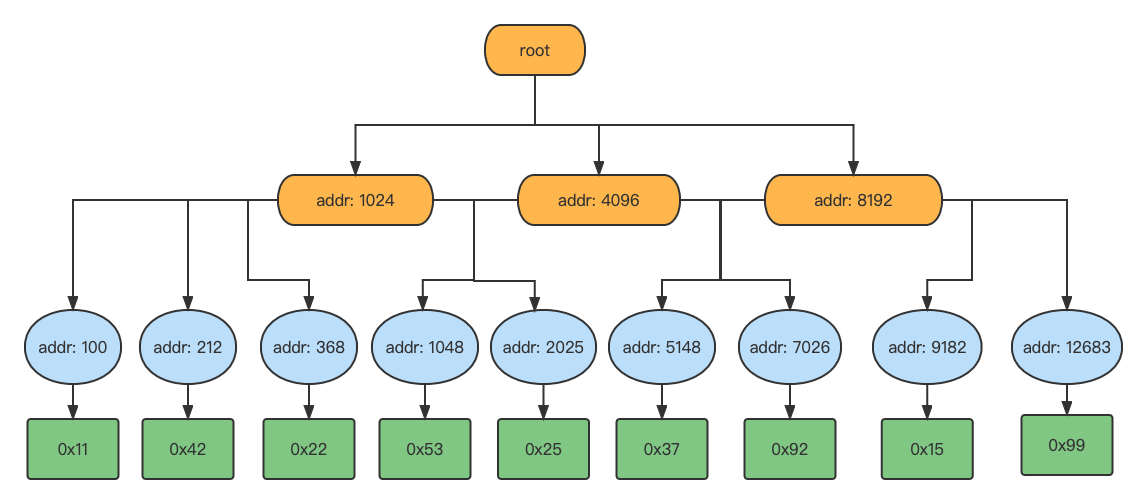
\includegraphics[width=0.8\textwidth]{memory-structure}
    \caption{OlaVM memory structure}
    \label{fig: B-tree-memory}
\end{figure}